\documentclass[a4paper]{article}

%use the english line for english reports
%usepackage[english]{babel}
\usepackage[portuguese]{babel}
\usepackage[utf8]{inputenc}
\usepackage{indentfirst}
\usepackage{graphicx}
\usepackage{verbatim}



%Todas as figuras devem ser referidas no texto. %\ref{fig:codigoFigura}
%
%%Exemplo de código para inserção de figuras
%%\begin{figure}[h!]
%%\begin{center}
%%escolher entre uma das seguintes três linhas:
%%\includegraphics[height=20cm,width=15cm]{path relativo da imagem}
%%\includegraphics[scale=0.5]{path relativo da imagem}
%%\includegraphics{path relativo da imagem}
%%\caption{legenda da figura}
%%\label{fig:codigoFigura}
%%\end{center}
%%\end{figure}
%
%
%\textit{Para escrever em itálico}
%\textbf{Para escrever em negrito}
%Para escrever em letra normal
%``Para escrever texto entre aspas''
%
%Para fazer parágrafo, deixar uma linha em branco.
%
%Como fazer bullet points:
%\begin{itemize}
	%\item Item1
	%\item Item2
%\end{itemize}
%
%Como enumerar itens:
%\begin{enumerate}
	%\item Item 1
	%\item Item 2
%\end{enumerate}
%
%\begin{quote}``Isto é uma citação''\end{quote}

\begin{document}

\setlength{\textwidth}{16cm}
\setlength{\textheight}{22cm}

\title{\Huge\textbf{Morelli}\linebreak\linebreak\linebreak
\Large\textbf{Relatório Final}\linebreak\linebreak
\linebreak\linebreak

\includegraphics[scale=0.1]{feup-logo.png}\linebreak\linebreak
\linebreak\linebreak
\Large{Mestrado Integrado em Engenharia Informática e Computação} \linebreak\linebreak
\Large{Programação em Lógica}\linebreak
}

\author{\textbf{Grupo xx:}\\ Francisco Rodrigues - Número 1 \\ Marta Lopes - 201208067 \\\linebreak\linebreak \\
 \\ Faculdade de Engenharia da Universidade do Porto \\ Rua Roberto Frias, s\/n, 4200-465 Porto, Portugal \linebreak\linebreak\linebreak
\linebreak\linebreak\vspace{1cm}}
%\date{Junho de 2007}
\maketitle
\thispagestyle{empty}

%************************************************************************************************
%************************************************************************************************

\newpage

\section*{Resumo}

\par Este trabalho teve como finalidade consolidar todo o conhecimento que fomos adquirindo na cadeira de PLOG e aplica-lo para criar um produto final. 
\par Como grupo podemos dizer que cooperamos bastante e trabalhamos sempre lado-a-lado, tornando todo o desenvolvimento do jogo mais fácil e fluido. 
\par \textit{Prolog} é uma linguagem de programação que se enquadra do paradigma da Programação em Lógica Matemática o que a torna um pouco diferente das linguagens a que estávamos habituados o que tornou mais difícil a resolução de pequenos problemas que felizmente foram sendo resolvidos com recurso à consulta dos materiais fornecidos pelos professores. Com isso conseguimos alcançar um jogo final não tão completo como o que gostaríamos que fosse no inicio, mas estamos contentes com o que conseguimos desenvolver apesar de tudo. 
\newpage

\tableofcontents

%************************************************************************************************
%************************************************************************************************

%*************************************************************************************************
%************************************************************************************************

\newpage

%%%%%%%%%%%%%%%%%%%%%%%%%%
\section{Introdução}

\par Para este projeto tínhamos como objetivo desenvolver um jogo em linha de comandos, como tal, decidimos escolher o \textit{Morelli} porque achamos que seria um jogo apelativo e interessante para desenvolver. De inicio o jogo parecia bastante simples, mas à medida que foi sendo desenvolvido notamos um certo aumento da dificuldade, no entanto nunca deixamos de perceber a dinâmica de jogo.
\par Reparamos em certas semelhanças com o jogo \textit{Othello} e \textit{Ming Mang} mas no geral o jogo que nós desenvolvemos é muito mais abstracto que todos os outros jogos de tabuleiro que conhecemos. Este trabalho serviu então para avaliar todos os nossos conhecimentos nesta linguagem nova para nós, e desenvolvendo este jogo que é completamente diferente daquilo a que estamos habituados.
\par Este relatório encontra-se dividido nas seguintes secções: 
\begin{itemize}
	\item História e regras de jogo;
	\item Implementação da lógica de jogo;
	\item Descrição da interface;
	\item Conclusões sobre este projeto;
	\item Bibliografia;
	\item Anexos, como o código do projeto.
\end{itemize}	


%%%%%%%%%%%%%%%%%%%%%%%%%%
\section{O Jogo XXX}

\par \textit{Morelli} é um jogo de tabuleiro criado por \textit{Richar Moxham} em 2011. É jogado por apenas 2 jogadores num tabuleiro de 13x13 quadrados em faixas concêntricas. A faixa de fora será a maior, com 48 casas, terminando na casa central. 

\begin{itemize}
	\item O jogo começa com \textbf{24 peças pretas} e \textbf{24 peças brancas}, ambas reversíveis, posicionadas nos quadrados de fora, de forma diametralmente oposta. Para além disso cada jogador vai ter \textbf{uma torre da cor respectiva}, que não vai entrar no tabuleiro no inicio do jogo. 
\begin{figure}[h!]
\begin{center}
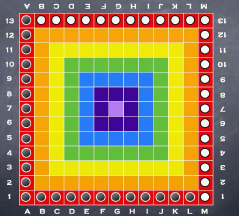
\includegraphics[scale=0.9]{fig1.png}
\caption{Inicio de Jogo}
\end{center}
\end{figure}

\item Cada jogador joga na sua vez, começando primeiro o jogador que tiver as peças da cor preta. Um \textbf{movimento legal} (Fig.2) consiste em mover a peça para um quadrado desocupado numa linha ortogonal ou diagonal desde que seja para uma faixa mais próxima do centro do que aquela em que se encontra no momento, não se podendo manter na mesma faixa ou voltar para trás (Fig.3).

\begin{figure}[h!]
\begin{center}
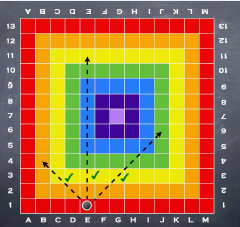
\includegraphics[scale=0.9]{fig2.png}
\caption{Movimento legal}
\end{center}
\end{figure}

\begin{figure}[h!]
\begin{center}
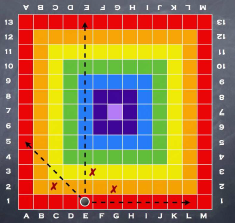
\includegraphics[scale=0.9]{fig3.png}
\caption{Movimento Ilegal}
\end{center}
\end{figure}

\newpage
\item Apenas será possivel passar pelo centro se este estiver vazio, não podendo parar nele. (Fig.4, Fig.5).

\begin{figure}[h!]
\begin{center}
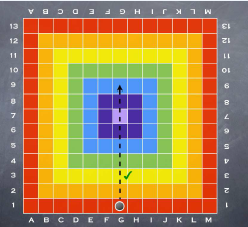
\includegraphics[scale=0.9]{center1.png}\linebreak\linebreak 
\caption{Movimento Legal}
\end{center}
\end{figure}

\begin{figure}[h!]
\begin{center}
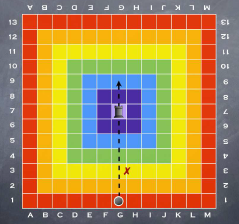
\includegraphics[scale=0.9]{center2.png}\linebreak\linebreak 
\caption{Movimento Ilegal}
\end{center}
\end{figure}


\newpage
\item A \textbf{captura do centro} é feita quando o jogador cria um quadrado de qualquer tamanho com as suas peças, centrado na célula central (Fig.4 e Fig.5). Quando o centro está capturado é colocada a torre da cor respectiva no centro do tabuleiro, removendo a torre adversária se se aplicar.


\begin{figure}[h!]
\begin{center}
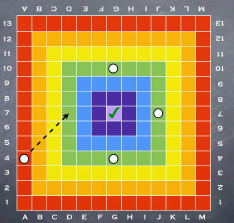
\includegraphics[scale=0.9]{fig4.png}
\caption{Captura do centro}
\end{center}
\end{figure}

\begin{figure}[h!]
\begin{center}
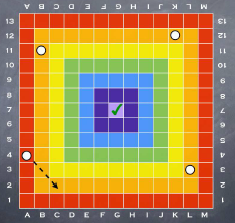
\includegraphics[scale=0.9]{fig41.png}
\caption{Captura do centro}
\end{center}
\end{figure}

\newpage
\item A cada movimento o jogador poderá \textbf{capturar uma peça adversária} quando conseguir rodea-la por duas peças da sua cor seja ortogonal ou diagonalmente (Fig.6). Uma peça capturada é revertida passando para a cor contrária. 

\begin{figure}[h!]
\begin{center}
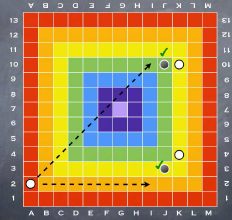
\includegraphics[scale=0.9]{fig5.png}
\caption{Captura de peça adversária}
\end{center}
\end{figure}


	\item O \textbf{vencedor} será o jogador que terá a sua torre no centro no final do jogo. O jogo acaba quando não existirem mais jogadas possíveis. Se o centro se mantiver sem nenhuma torre até ao final do jogo, é um empate. 

\end{itemize}



%%%%%%%%%%%%%%%%%%%%%%%%%%
\section{Lógica do Jogo}

Descrever o projeto e implementação da lógica do jogo em Prolog, incluindo a forma de representação do estado do tabuleiro e sua visualização, execução de movimentos, verificação do cumprimento das regras do jogo, determinação do final do jogo e cálculo das jogadas a realizar pelo computador utilizando diversos níveis de jogo. Sugere-se a estruturação desta secção da seguinte forma:

\subsection{Representação do Estado do Jogo} Pode ser idêntico ao descrito no relatório intercalar.)

\subsection{Visualização do Tabuleiro} (Pode ser idêntico ao descrito no relatório intercalar.)

\subsection{Lista de Jogadas Válidas} Obtenção de uma lista de jogadas possíveis. Exemplo: \textit{valid\_moves(+Board, -ListOfMoves)}.

\subsection{Execução de Jogadas} Validação e execução de uma jogada num tabuleiro, obtendo o novo estado do jogo. Exemplo: \textit{move(+Move, +Board, -NewBoard)}.

\subsection{Avaliação do Tabuleiro} Avaliação do estado do jogo, que permitirá comparar a aplicação das diversas jogadas disponíveis. Exemplo: \textit{value(+Board, +Player, -Value)}.

\subsection{Final do Jogo} Verificação do fim do jogo, com identificação do vencedor. Exemplo: \textit{game\_over(+Board, -Winner)}.

\subsection{Jogada do Computador} Escolha da jogada a efetuar pelo computador, dependendo do nível de dificuldade. Por exemplo: \textit{choose\_move(+Level, +Board, -Move)}.


%%%%%%%%%%%%%%%%%%%%%%%%%%
\section{Interface com o Utilizador}

Descrever o módulo de interface com o utilizador em modo de texto.


%%%%%%%%%%%%%%%%%%%%%%%%%%
\section{Conclusões}
Que conclui deste projecto? Como poderia melhorar o trabalho desenvolvido?


\clearpage
\addcontentsline{toc}{section}{Bibliografia}
\renewcommand\refname{Bibliografia}
\bibliographystyle{plain}
\bibliography{myrefs}
\par "Morelli." BoardGameGeeks. N.p., 2011. Web. 2015.
\par "Morelli at Boardspace.net"  Boardspace.net. N.p., 2011. Web. 2015.

\newpage
\appendix
\section{Nome do Anexo}
Código Prolog implementado devidamente comentado e outros elementos úteis que não sejam essenciais ao relatório.

\end{document}
